\documentclass[12pt]{article}

\usepackage{lmodern}
\usepackage[colorlinks = true,
            linkcolor = blue,
            urlcolor = blue]{hyperref}
\usepackage{graphicx}
\begin{document}

\section{Basic Info}
\begin{description}
    \item [Project Title]  Curly Squeegee goes to Hollywood 
    \item [Names]  Brian Kimmig, Jimmy Moore
    \item[e-mail] brian.kimmig@utah.edu, jimmy@cs.utah.edu
    \item [uID] u0560080, u1012009
    \item [Project Github] \href{https://github.com/bkimmig/curly-squeegee-6630}{curly-squeegee-6630}
\end{description}


\section{Background \& Motivation}
\textit{Discuss your motivations and reasons for choosing this project, especially any background or research interests that may have influenced your decision.}

Both of us watch a fair amount of movies and find ourselves looking at sites like \href{www.imdb.com}{IMDB} and wanting to see the scope of an actors career through more than text, and more than one parameter at a time.

We are choosing to look at actors careers through visualization because movies and their casts are relate-able to large groups of people with minimal explanation. This semi-dynamic dataset has a large appeal because users have the freedom to learn about the actor of their choice and movies through visualization. 

For our project, we want to visually represent the career arc of actors as measured by number of movies, ratings, earnings, spouses as gathered from \href{www.imdb.com}{IMDB} and other sites (mentioned below). 

We want to see the textual data with high dimensionality in an easy to digest manner.  


\section{Project Objectives}
Provide the primary questions you are trying to answer with your visualization. 
\begin{itemize}

    \item  {\it What would you like to learn and accomplish?}
    We want to look for trends in actors careers over time with respect to film rating, number of movies a year, estimated salary. Also who they have worked with and how that has affected their careers.

    \item  {\it List benefits of your project}
    A single place that aggregates data about actors careers from multiple sites and allows a user to visualize it in multiple ways. We don't know if anything will pop out but it invites people to look and ask questions about our favorite celebrities.  

\end{itemize}

\section{Data}
\begin{enumerate}
    \item Where did you get the data?
        We will be pulling data from a few APIs on the Internet. We have set up web framework using node.js and Meteor that uses a RESTful archetecture to gather data from APIs on the web via GET requests. This data is stored in a MongoDB database.
    
    \item how did you get the data?
        Our data will be dynamic, so based on the actor the person wants to learn about we will query an API to gather the info. 
    
    \item links to data-sources:
    \begin{itemize}
        \item \href{http://www.myapifilms.com/}{My API Films}
        \item \href{www.omdbapi.com}{OMdb}
    \end{itemize}
\end{enumerate}

\section{Data Processing}
\begin{description}
    
    \item [Formatting] Do you expect to do substantial data clean-up?
        
        Not too much clean-up as the data comes in JSON format from the API.  The data returned from an actor is fairly detailed, so we plan to cull and aggregate the data based on what we plan to visualize and also to make it easier to pass to our views.   
        We will create the following tables:  
        \begin{itemize}
        \item \textbf{Actors Table:} This will store all data on our selected actor, including the movies they have acted in.
        \item \textbf{Movies Table:}  will contain all of the information for each movie we wish to plot or visualize.  We will also add genre counts for each film for our force directed genre diagram.
		\end{itemize}        
     

    \item [Dimensions] What quantities do you plan to derive from your data?

        We will want to derive means, medians, standard deviations of the quantitative data, and maintain genre counts of the various films in the actor's filmography.   
        

    \item [Method] How will data processing be implemented?

        Using built in math functions and basic statistical analysis and aggregate counts of parameters in JS. 

\end{description}
  
  
\section{Visualization Design}
\begin{description}
\item [Presentation]  How will you display your data? Provide some general ideas that you have for the visualization design. Develop three alternative prototype designs for your visualization. Create one final design that incorporates the best of your three designs. Describe your designs and justify your choices of visual encodings. We recommend you use the Five Design Sheet Methodology.
\end{description}
  
  Below, we discuss our visual designs and the rationale behind our choices.  We find The following three visualizations we present to be the most effective method of showcasing an actor's career.
\section{Must-Have Features}

List the features without which you would consider your project to be a failure.

See below.

\section{Optional Features}
See below.
 

\newpage

\section{Desigh Criteria}

\subsection{Landing Page}
\begin{center}
 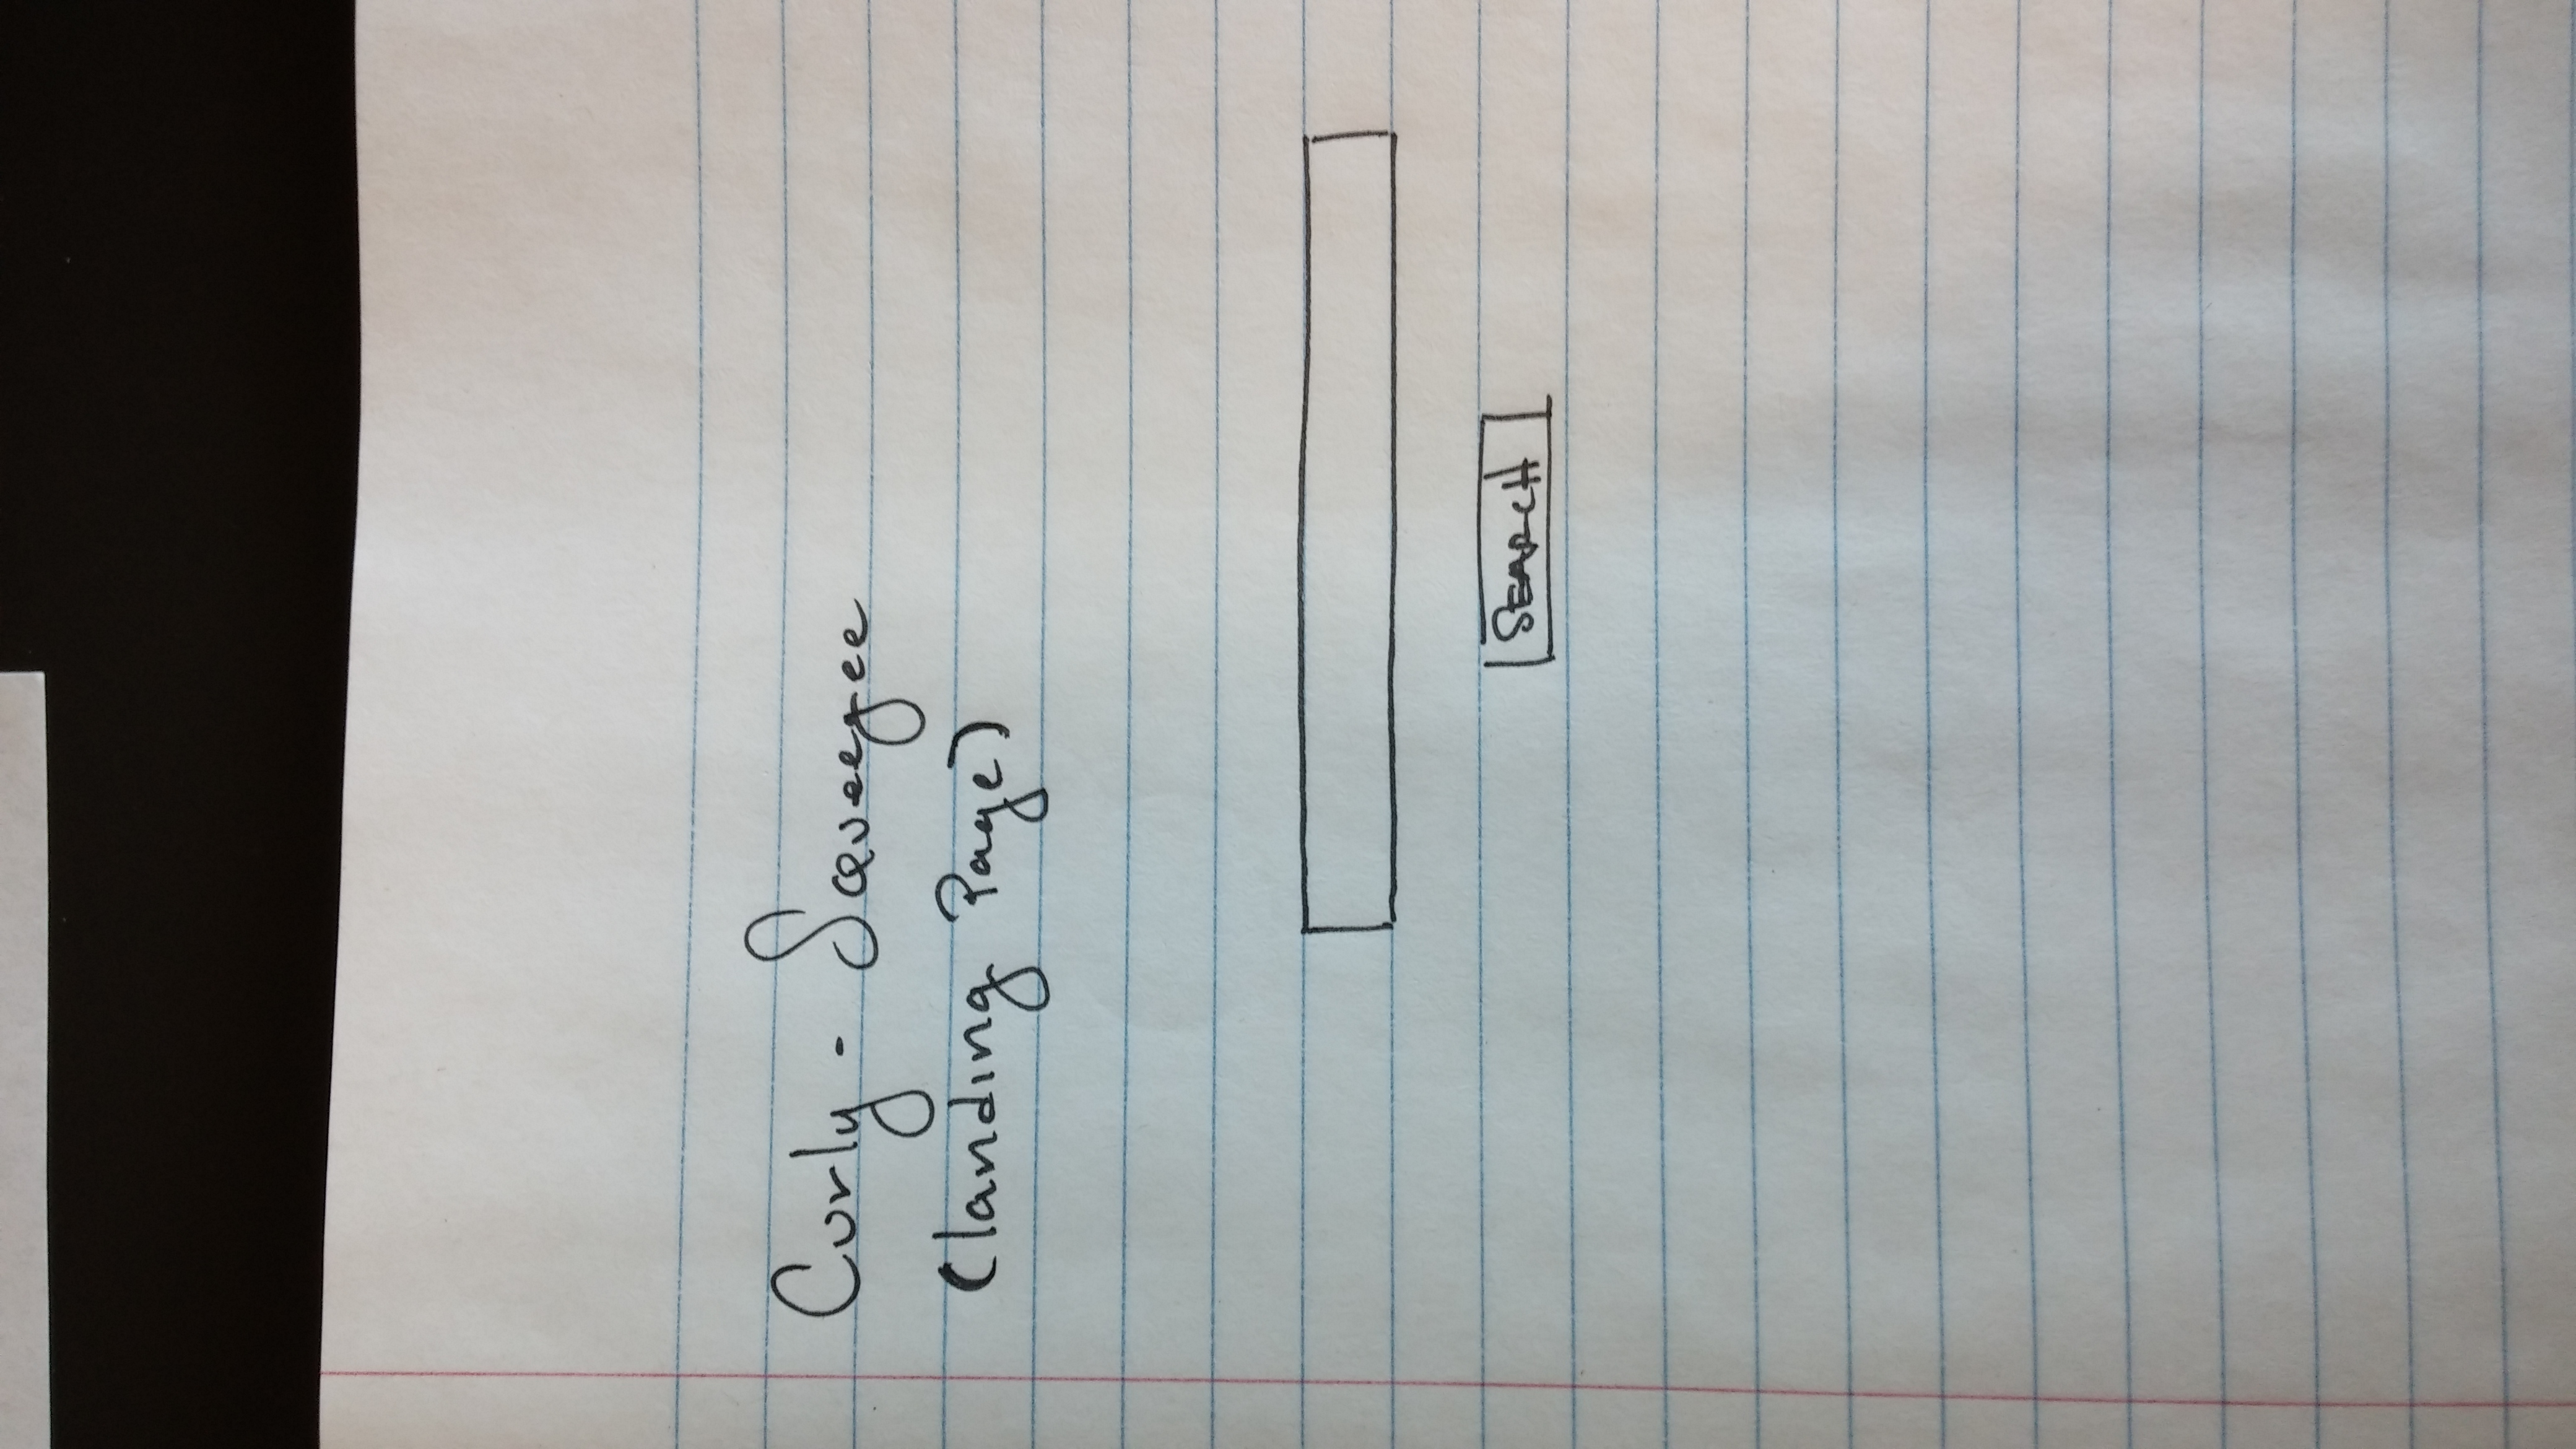
\includegraphics[angle=-90,scale=0.05]{landing}
\end{center}
 This is the first screen the user sees.  Our goal is to provide a familiar google-esque page layout with text field, search button, and Project name "curly squeegee" prominently displayed
 
 \vspace{2em}
 
 \textbf{Mandatory Features}
 \begin{itemize}
  	\item Minimal welcome text and instruction
  	\item Text box
  	\item search button
 \end{itemize}

 \vspace{2em}
 \textbf{Optional Features}
\begin{itemize}
\item graphic designed logo
	\item Random actor button
	\item list of currently popular actors as scraped from current releases
\end{itemize}

\newpage

\subsection{Loading Screen}

%\begin{center}
% 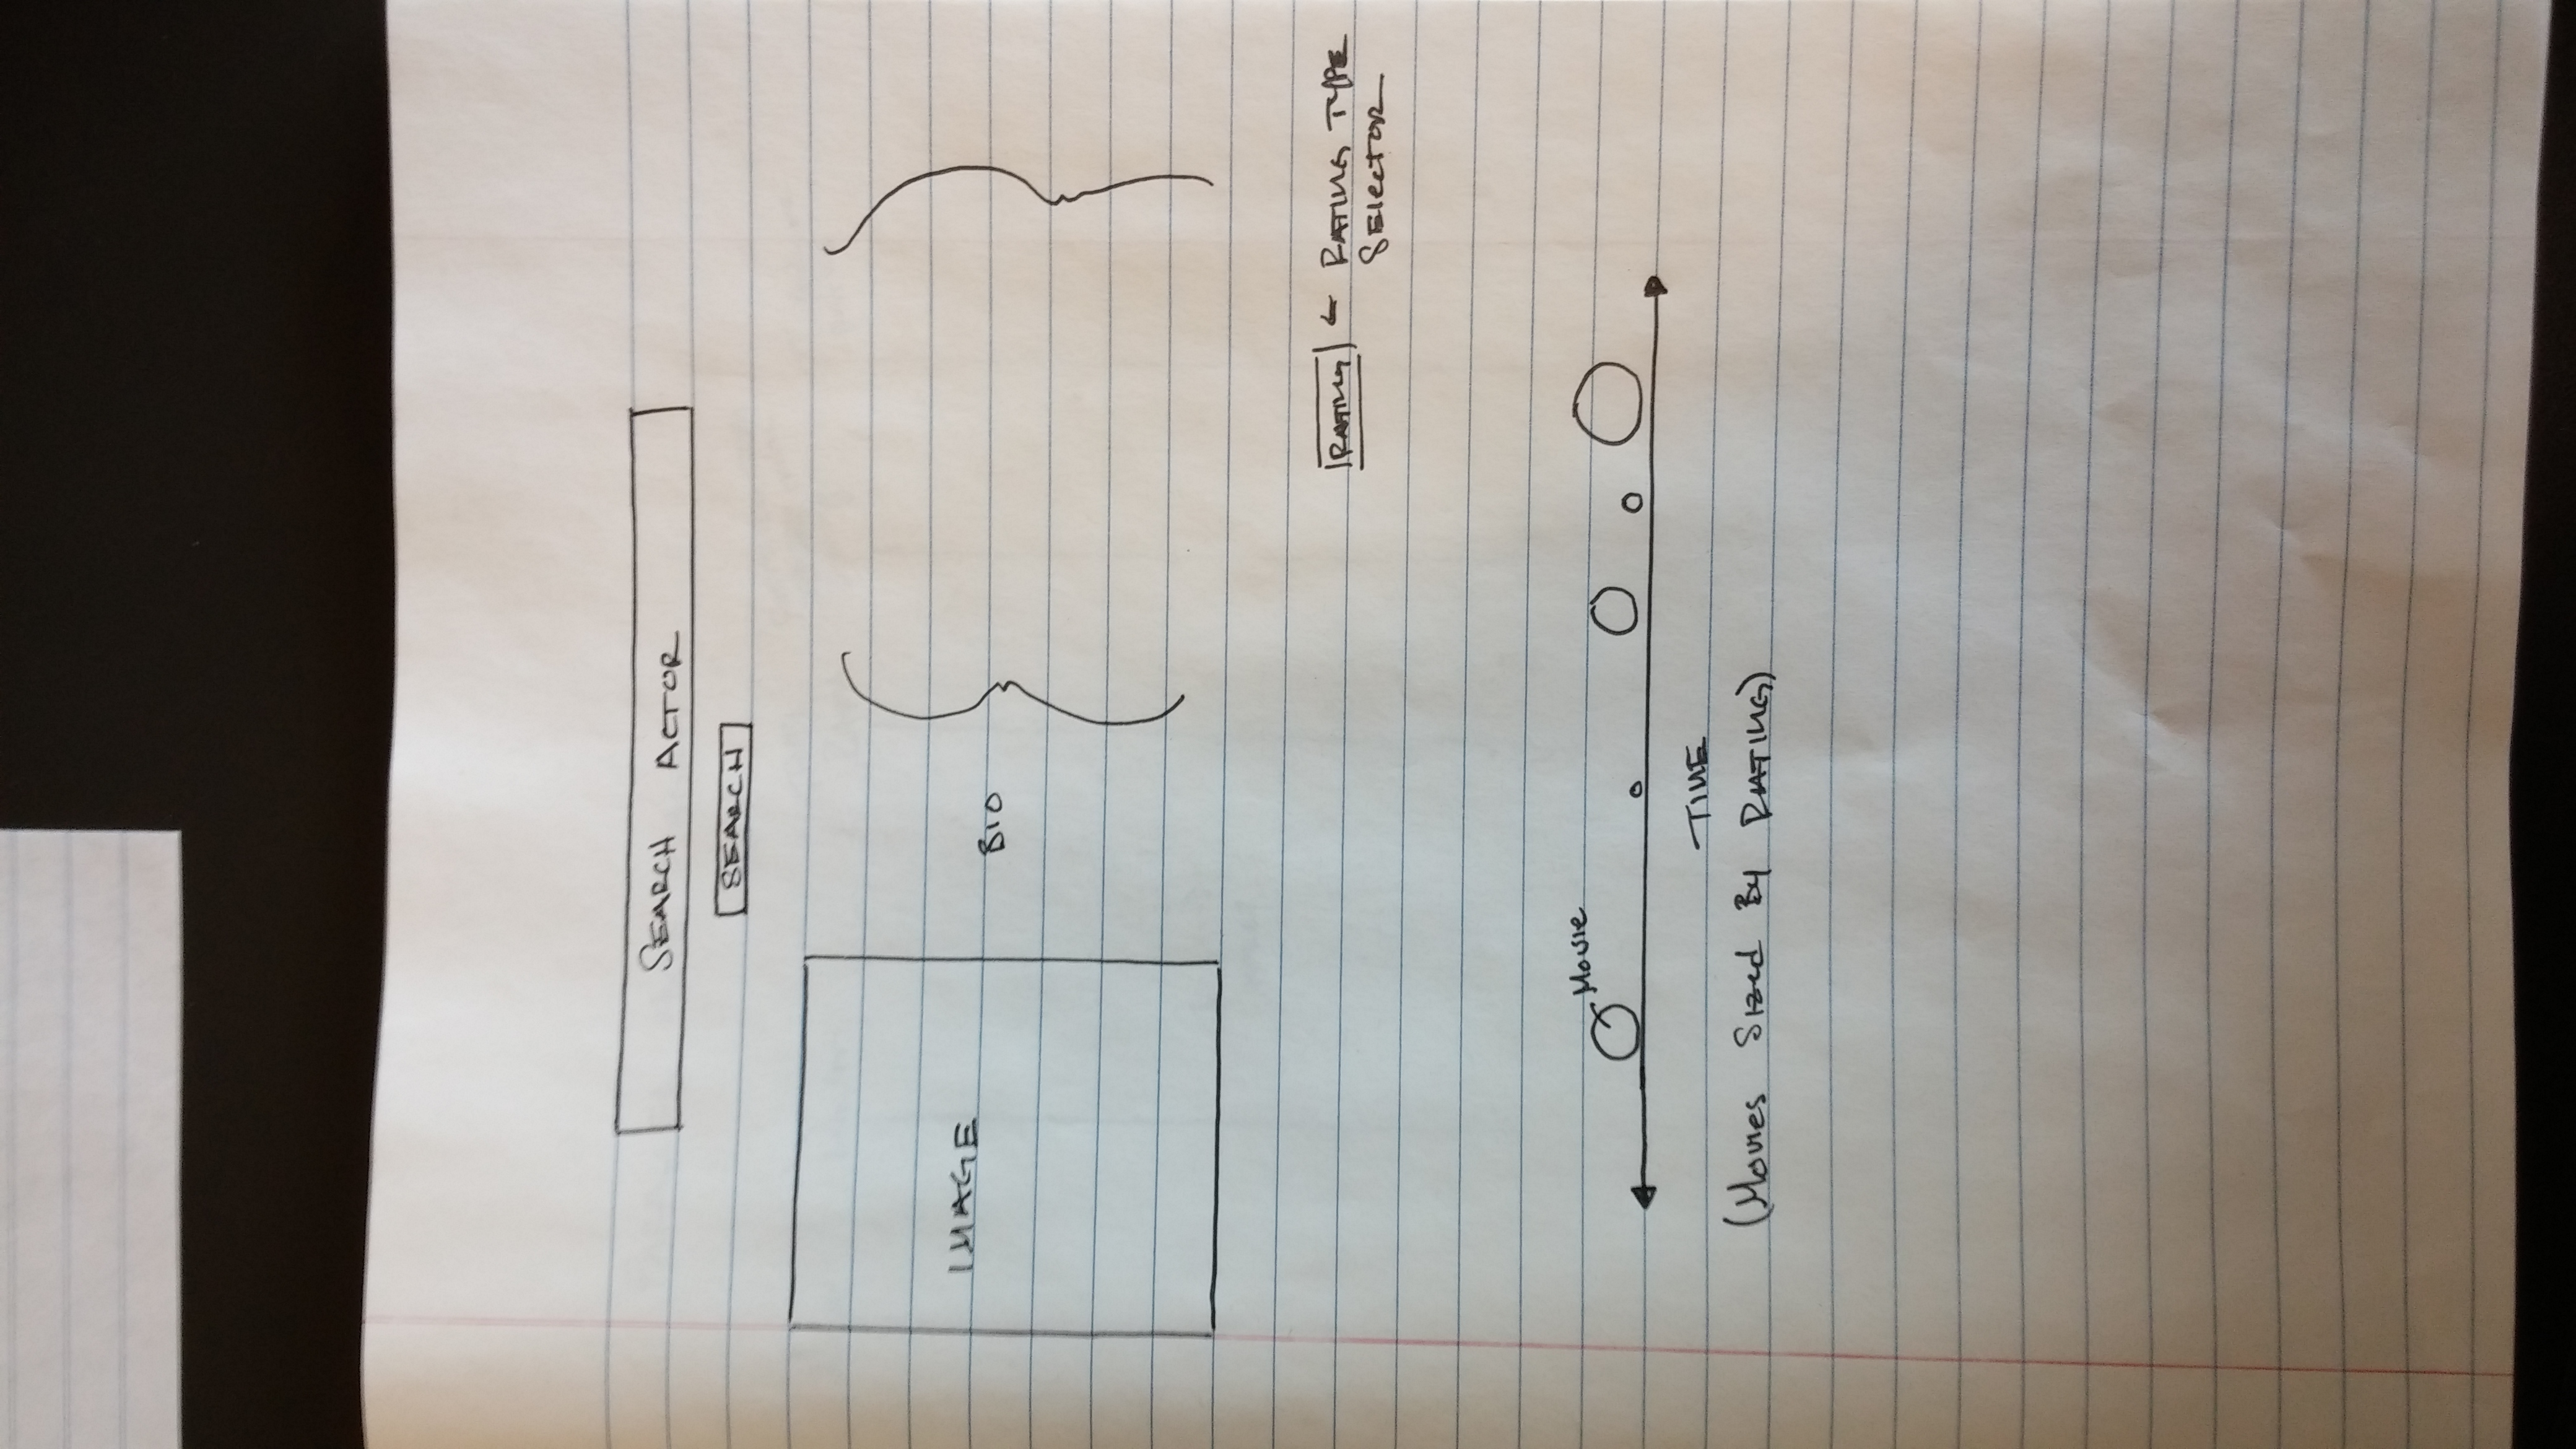
\includegraphics[scale=0.5]{main.jpg}
%\end{center}

 After the user enters a text input, the screen state should change (perhaps darken or fade?) and display a dynamic loading icon.
 
 \vspace{2em}
 
 \textbf{Mandatory Features}
 \begin{itemize}
  	\item Display "Fetching Actor filmography" or similar static message
  	\item Dynamic loading icon 
 \end{itemize}

 \vspace{2em}
 \textbf{Optional Features}
\begin{itemize}

	\item Screen darkens or fades	
	\item Live updates on what is currently being queried or fetched
	\item some type of loading bar
\end{itemize}
	
\newpage

\subsection{Main Screen}
\begin{center}
 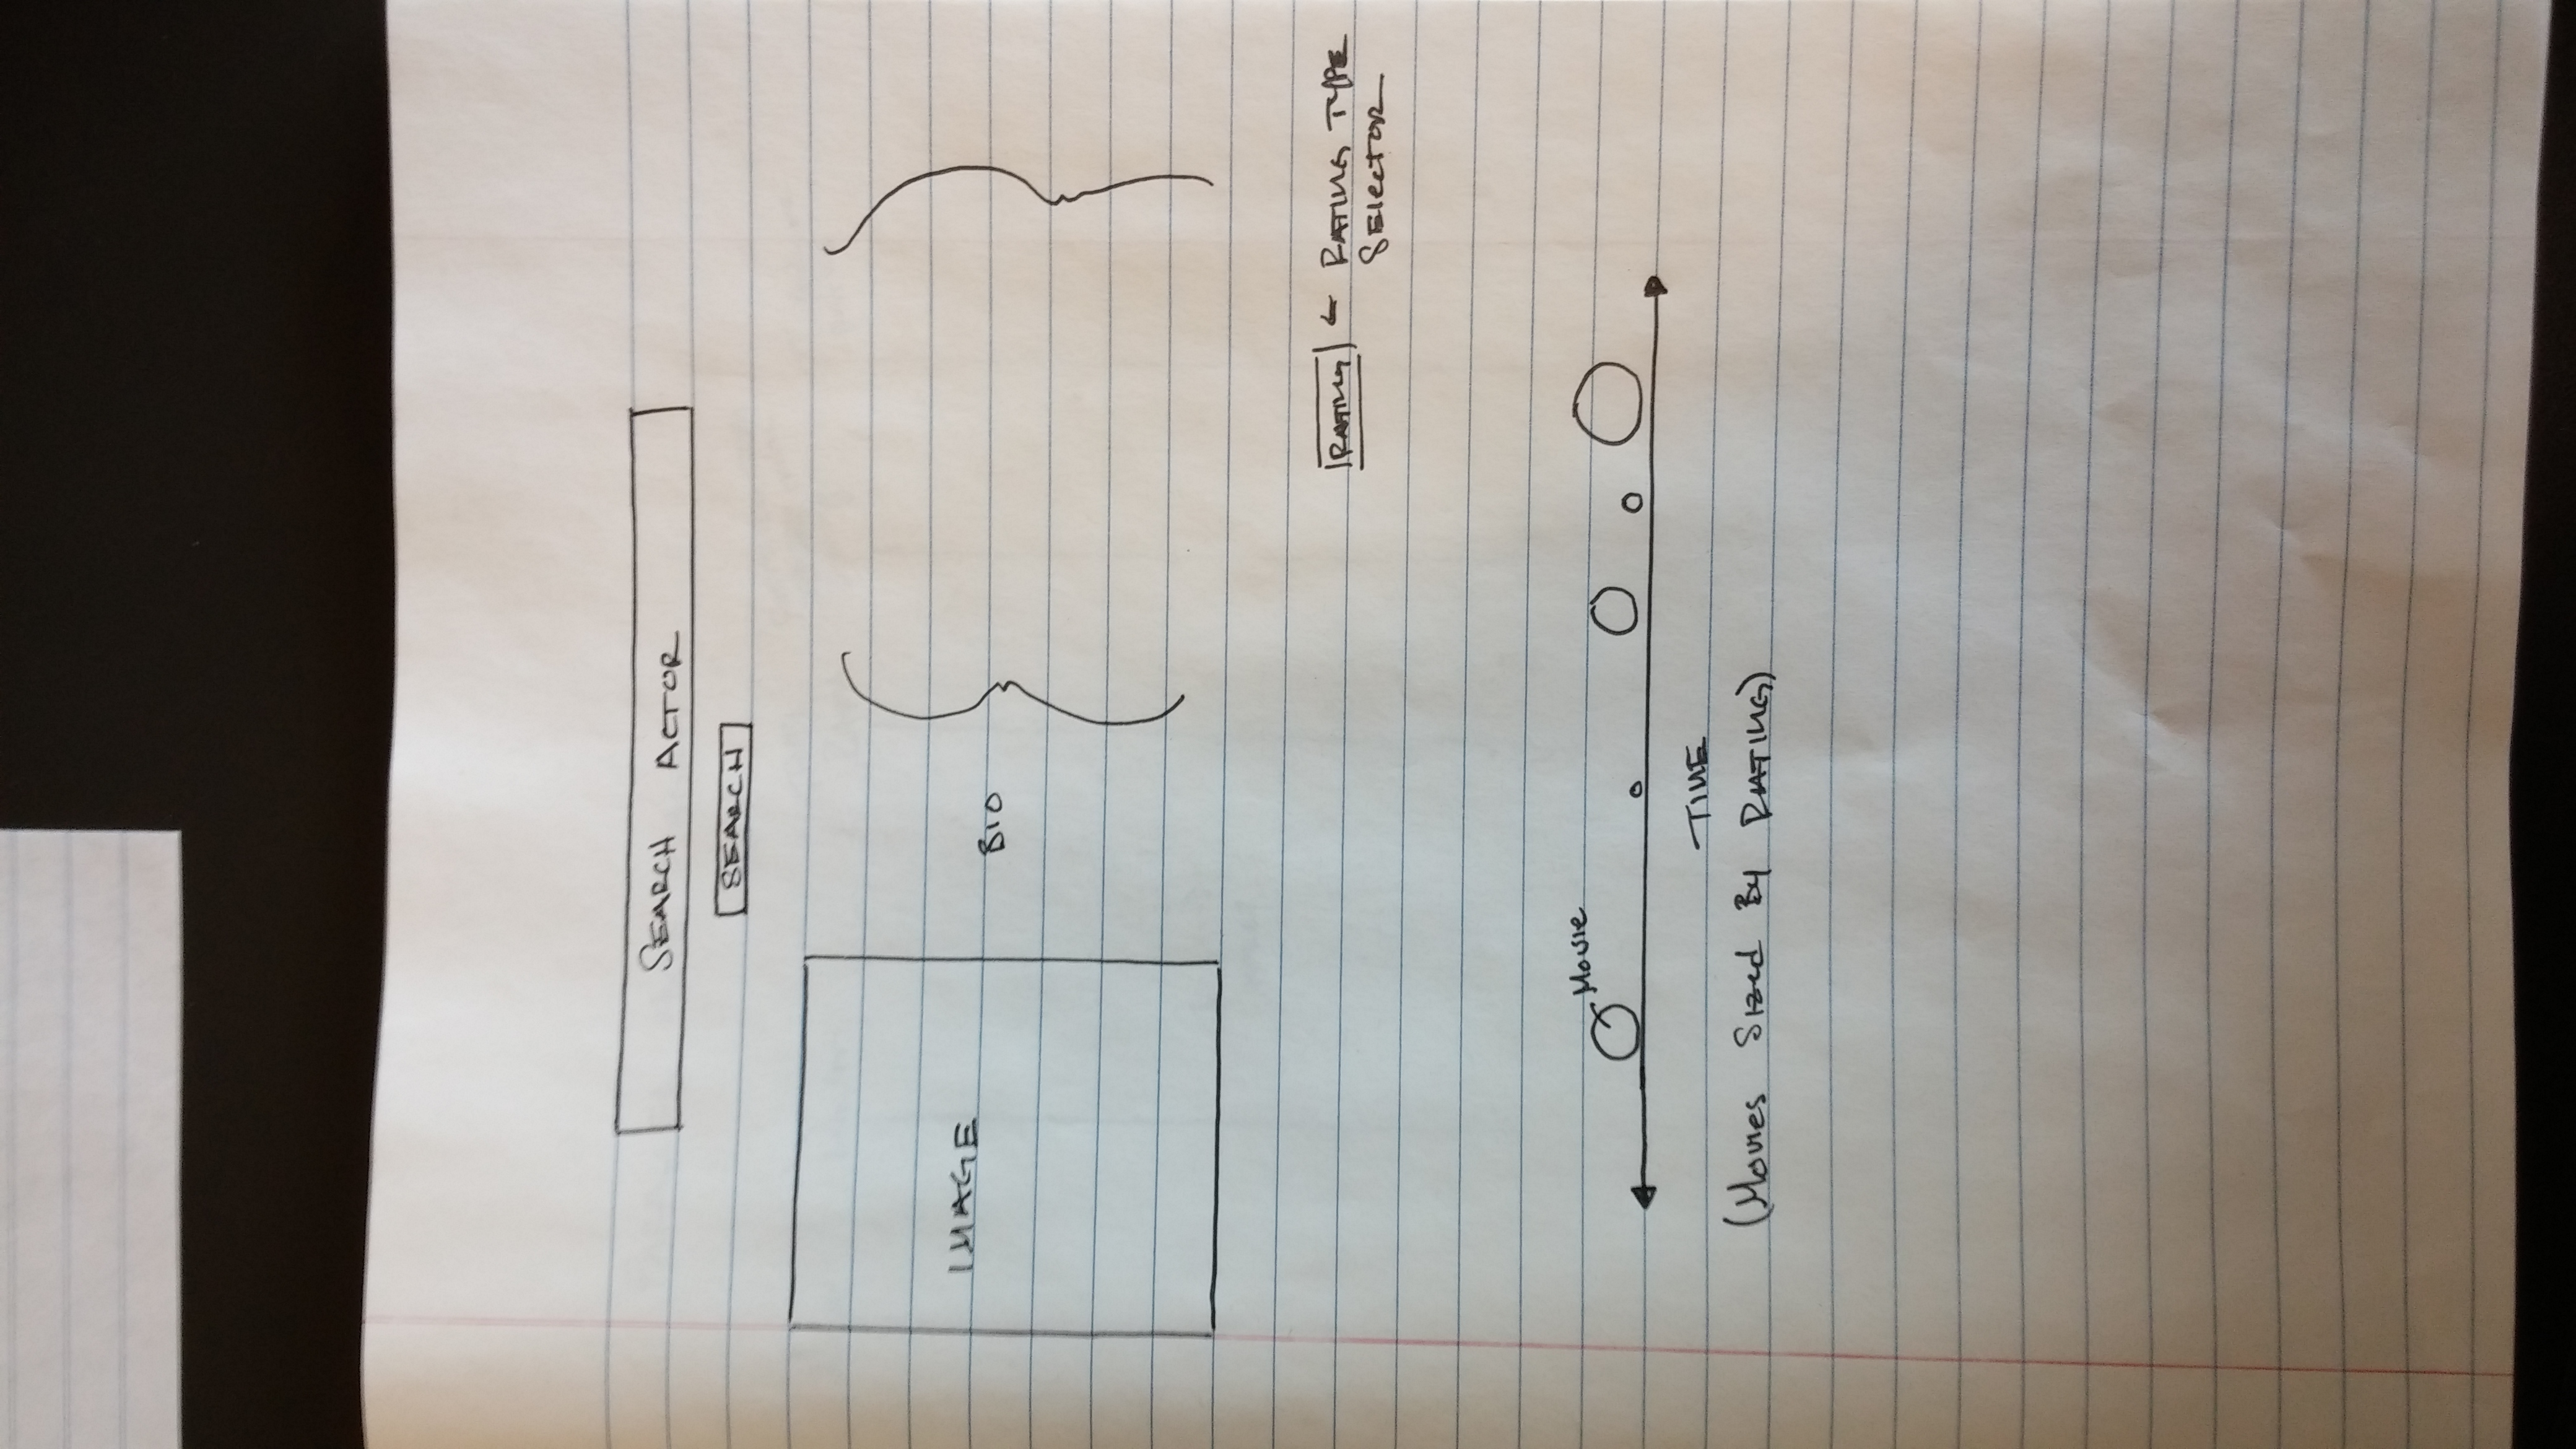
\includegraphics[angle=-90,scale=0.05]{main.jpg}
\end{center}
 Once the Actor information has been obtained, parsed, and stored in our database, we will display a brief Bio.  
 Displaying this information servers two purposes.  One, It gives context to the data, and two, it is a simple way to let the user know whether they are seeing information for the right actor.  For instance, Nic Cage is a separate actor from Nicolas Cage.
 
 \vspace{2em}
 
 \textbf{Mandatory Features}
 \begin{itemize}
  	\item Actor photo
  	\item Actor Bio
  	\begin{itemize}
  		\item Name
  		\item Birth Date
  		\item Years Active
  		\item Number of Films
  		\item etc.
  	\end{itemize}
  	
 \end{itemize}

\vspace{2em}
 
 \textbf{Optional Features}
\begin{itemize}
	\item Disambiguation ( but don't hold your breath)
\end{itemize}
\subsubsection{Career Timeline}
This graph shows the selected actors entire filmography as a timeline, with each film represented as a circle, sized by film rating (rating selection TBD). This timeline represents the best of our previous design iterations (drill-down barchart, pie chart), and we feel conveys the actor's career most naturally.  At a glance, we can determine the critical merit of the body of their work, as well as thier acting output over their career.

\vspace{2em}
\textbf{Mandatory Features}
\begin{itemize}
 	\item Circle sizing by film rating
 	\item Hover text for each film
 		\begin{itemize}
 			\item film title
 			\item plot summary
 			\item ratings
 		\end{itemize}

 \end{itemize} 
 
 \textbf{Optional Features}
\begin{itemize}
\item 	Film poster on hover 
\item Circle fill color based on genre
\item zoomable timeline
\end{itemize}
\newpage

\subsection{Parallel Axis Diagram}
\begin{center}
 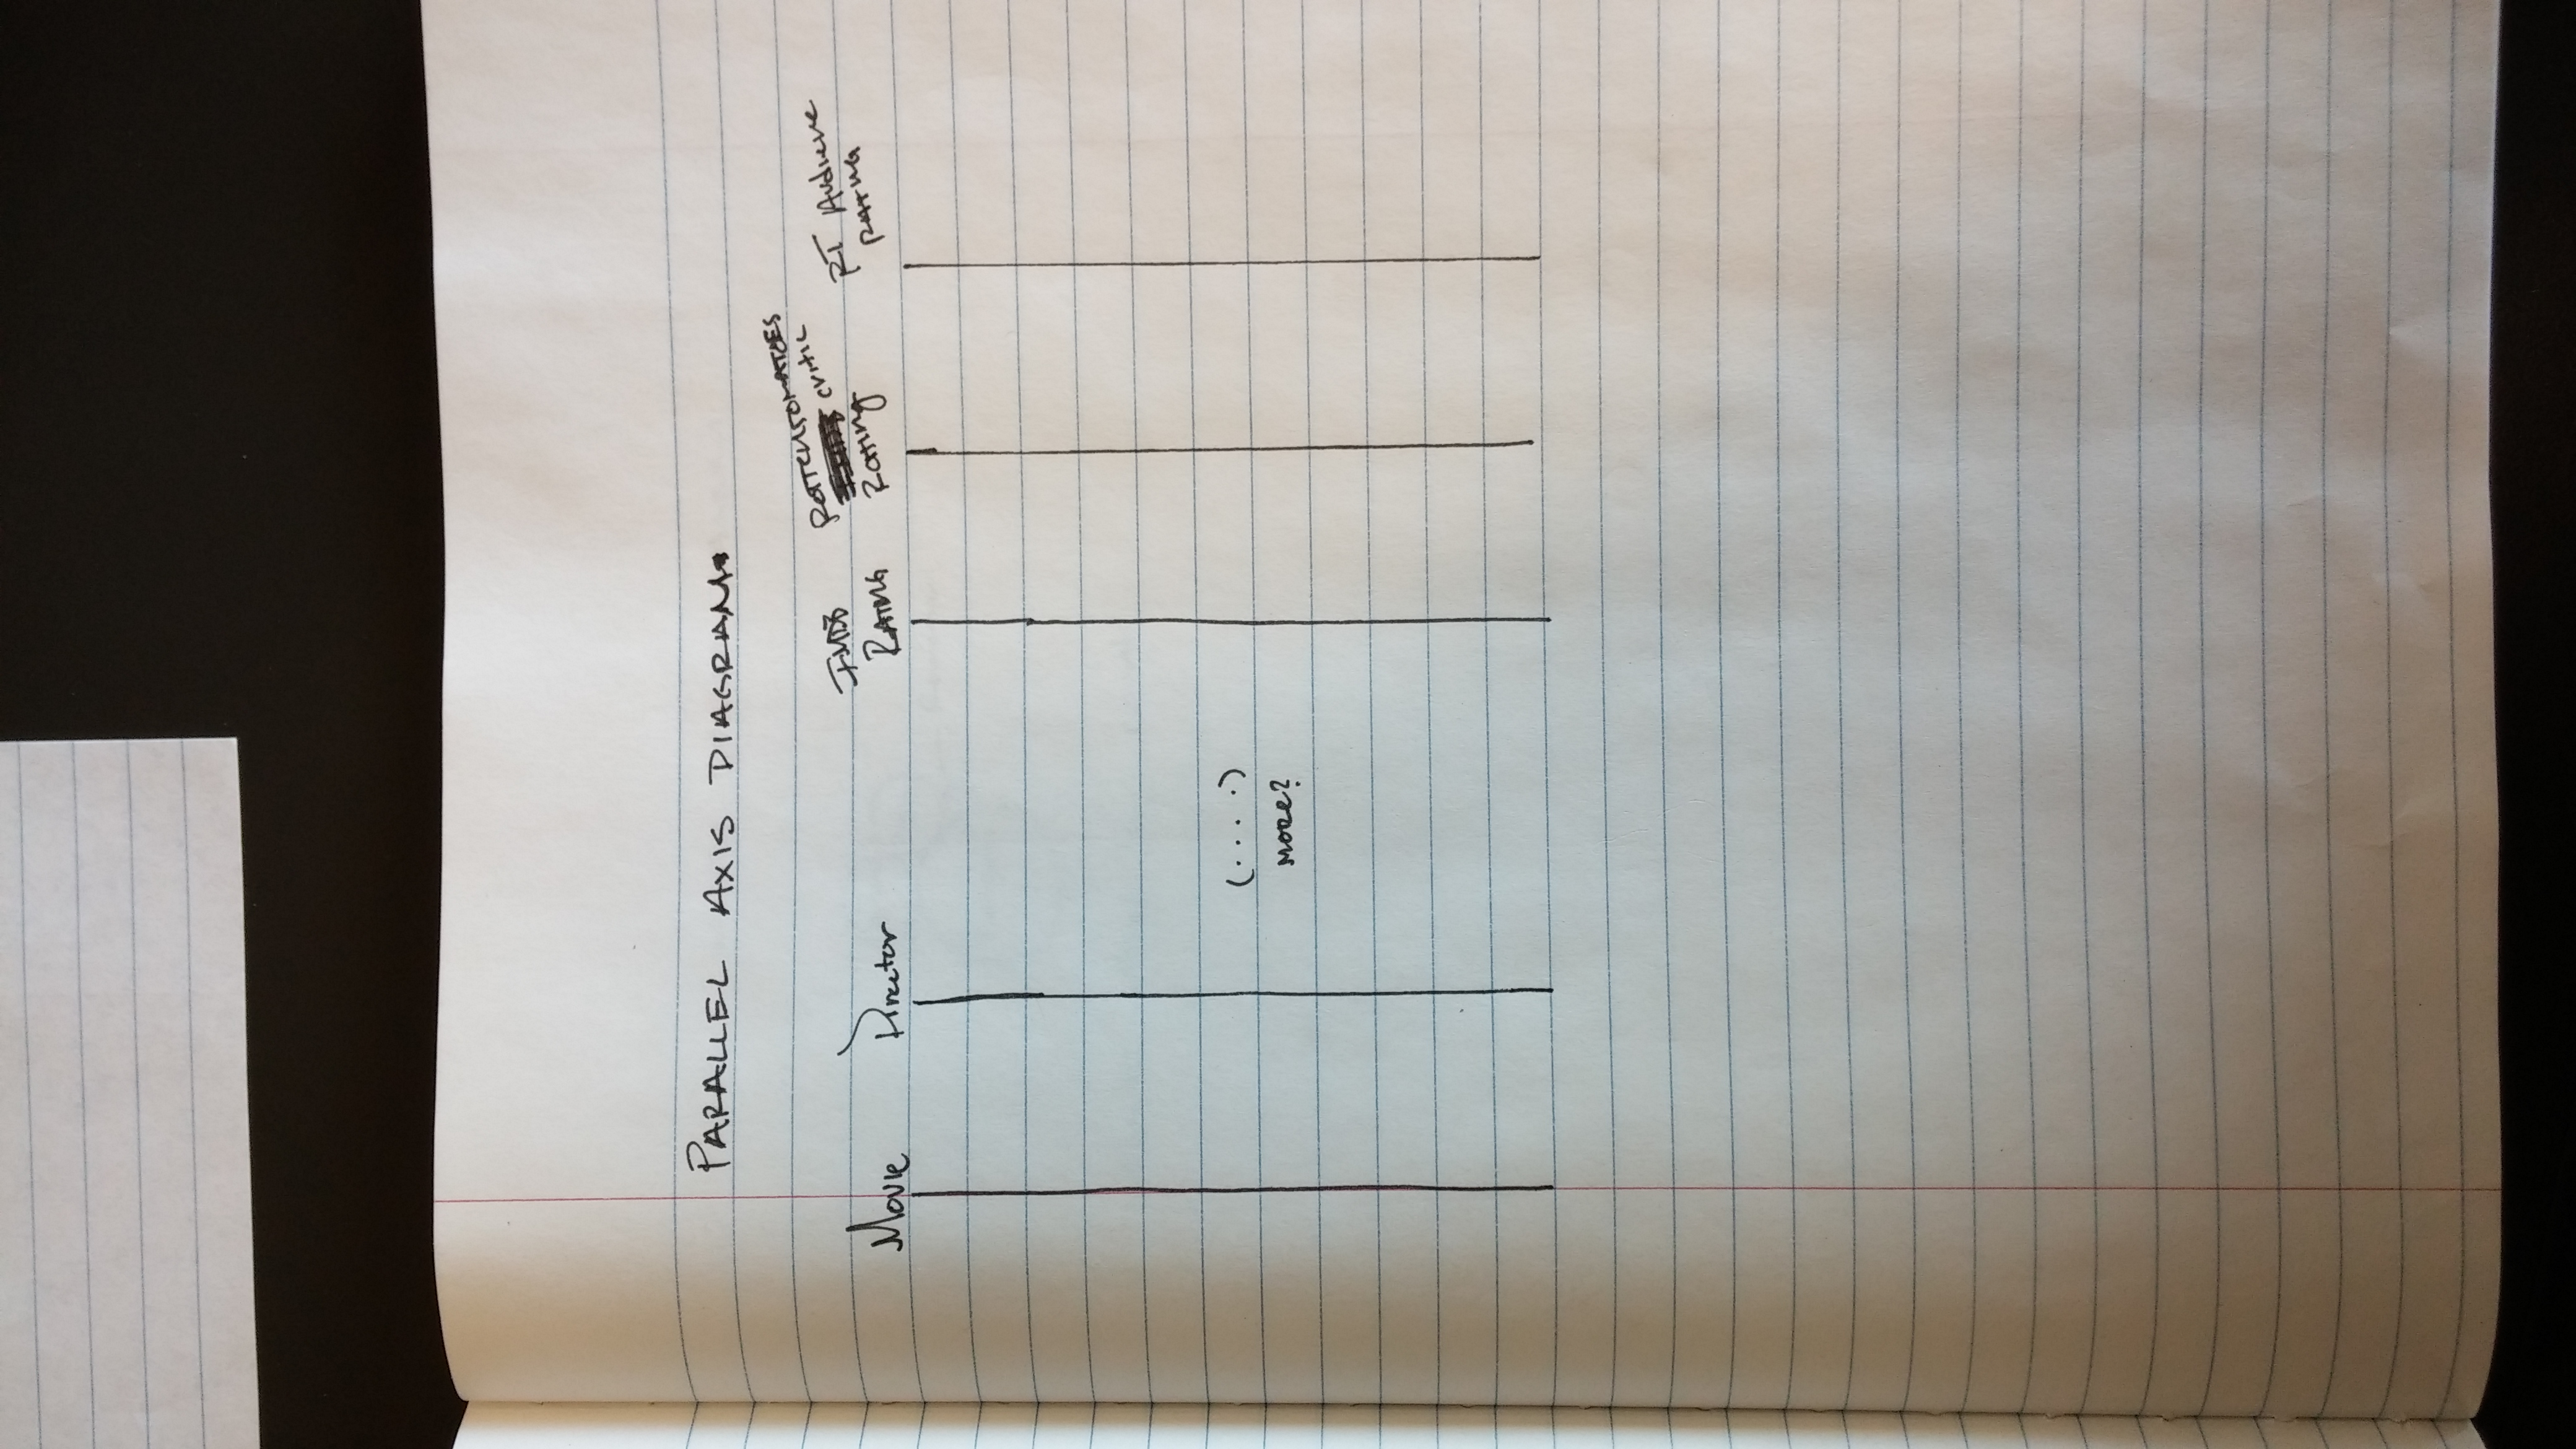
\includegraphics[angle=-90, scale=0.05]{parallel.jpg}
\end{center}
 This presents a large collection of filmography data for the user to explore based on their own search criteria.  Incorporating a parallel axis diagram reduces the number of individual plots we originally wanted to show.  It combines multiple parameter groupings  in one view allowing us to explore several variables at once. 
 
 Prospective axes include:
 
 \begin{itemize}
	\item Actors (Top-billed) 
 	\item Film Title
 	\item Years
 	\item Director
 	\item Rating
 		\begin{itemize}
 			\item IMDB Rating
 			\item Rotten Tomatoes Critical rating
 			\item Rotten Tomatoes user rating
 		\end{itemize}
 \end{itemize}
 
 
 \vspace{2em}
 
 \textbf{Mandatory Features}
 \begin{itemize}
 	\item brushing enabled on all axes
 	\item Highlighting corresponding selected films
 	\item hovering on crowded text
  	
 \end{itemize}

\vspace{2em}
 
 \textbf{Optional Features}
\begin{itemize}
	\item N/A
\end{itemize}


\newpage

\subsection{Force Directed Genre Diagram}
\begin{center}
 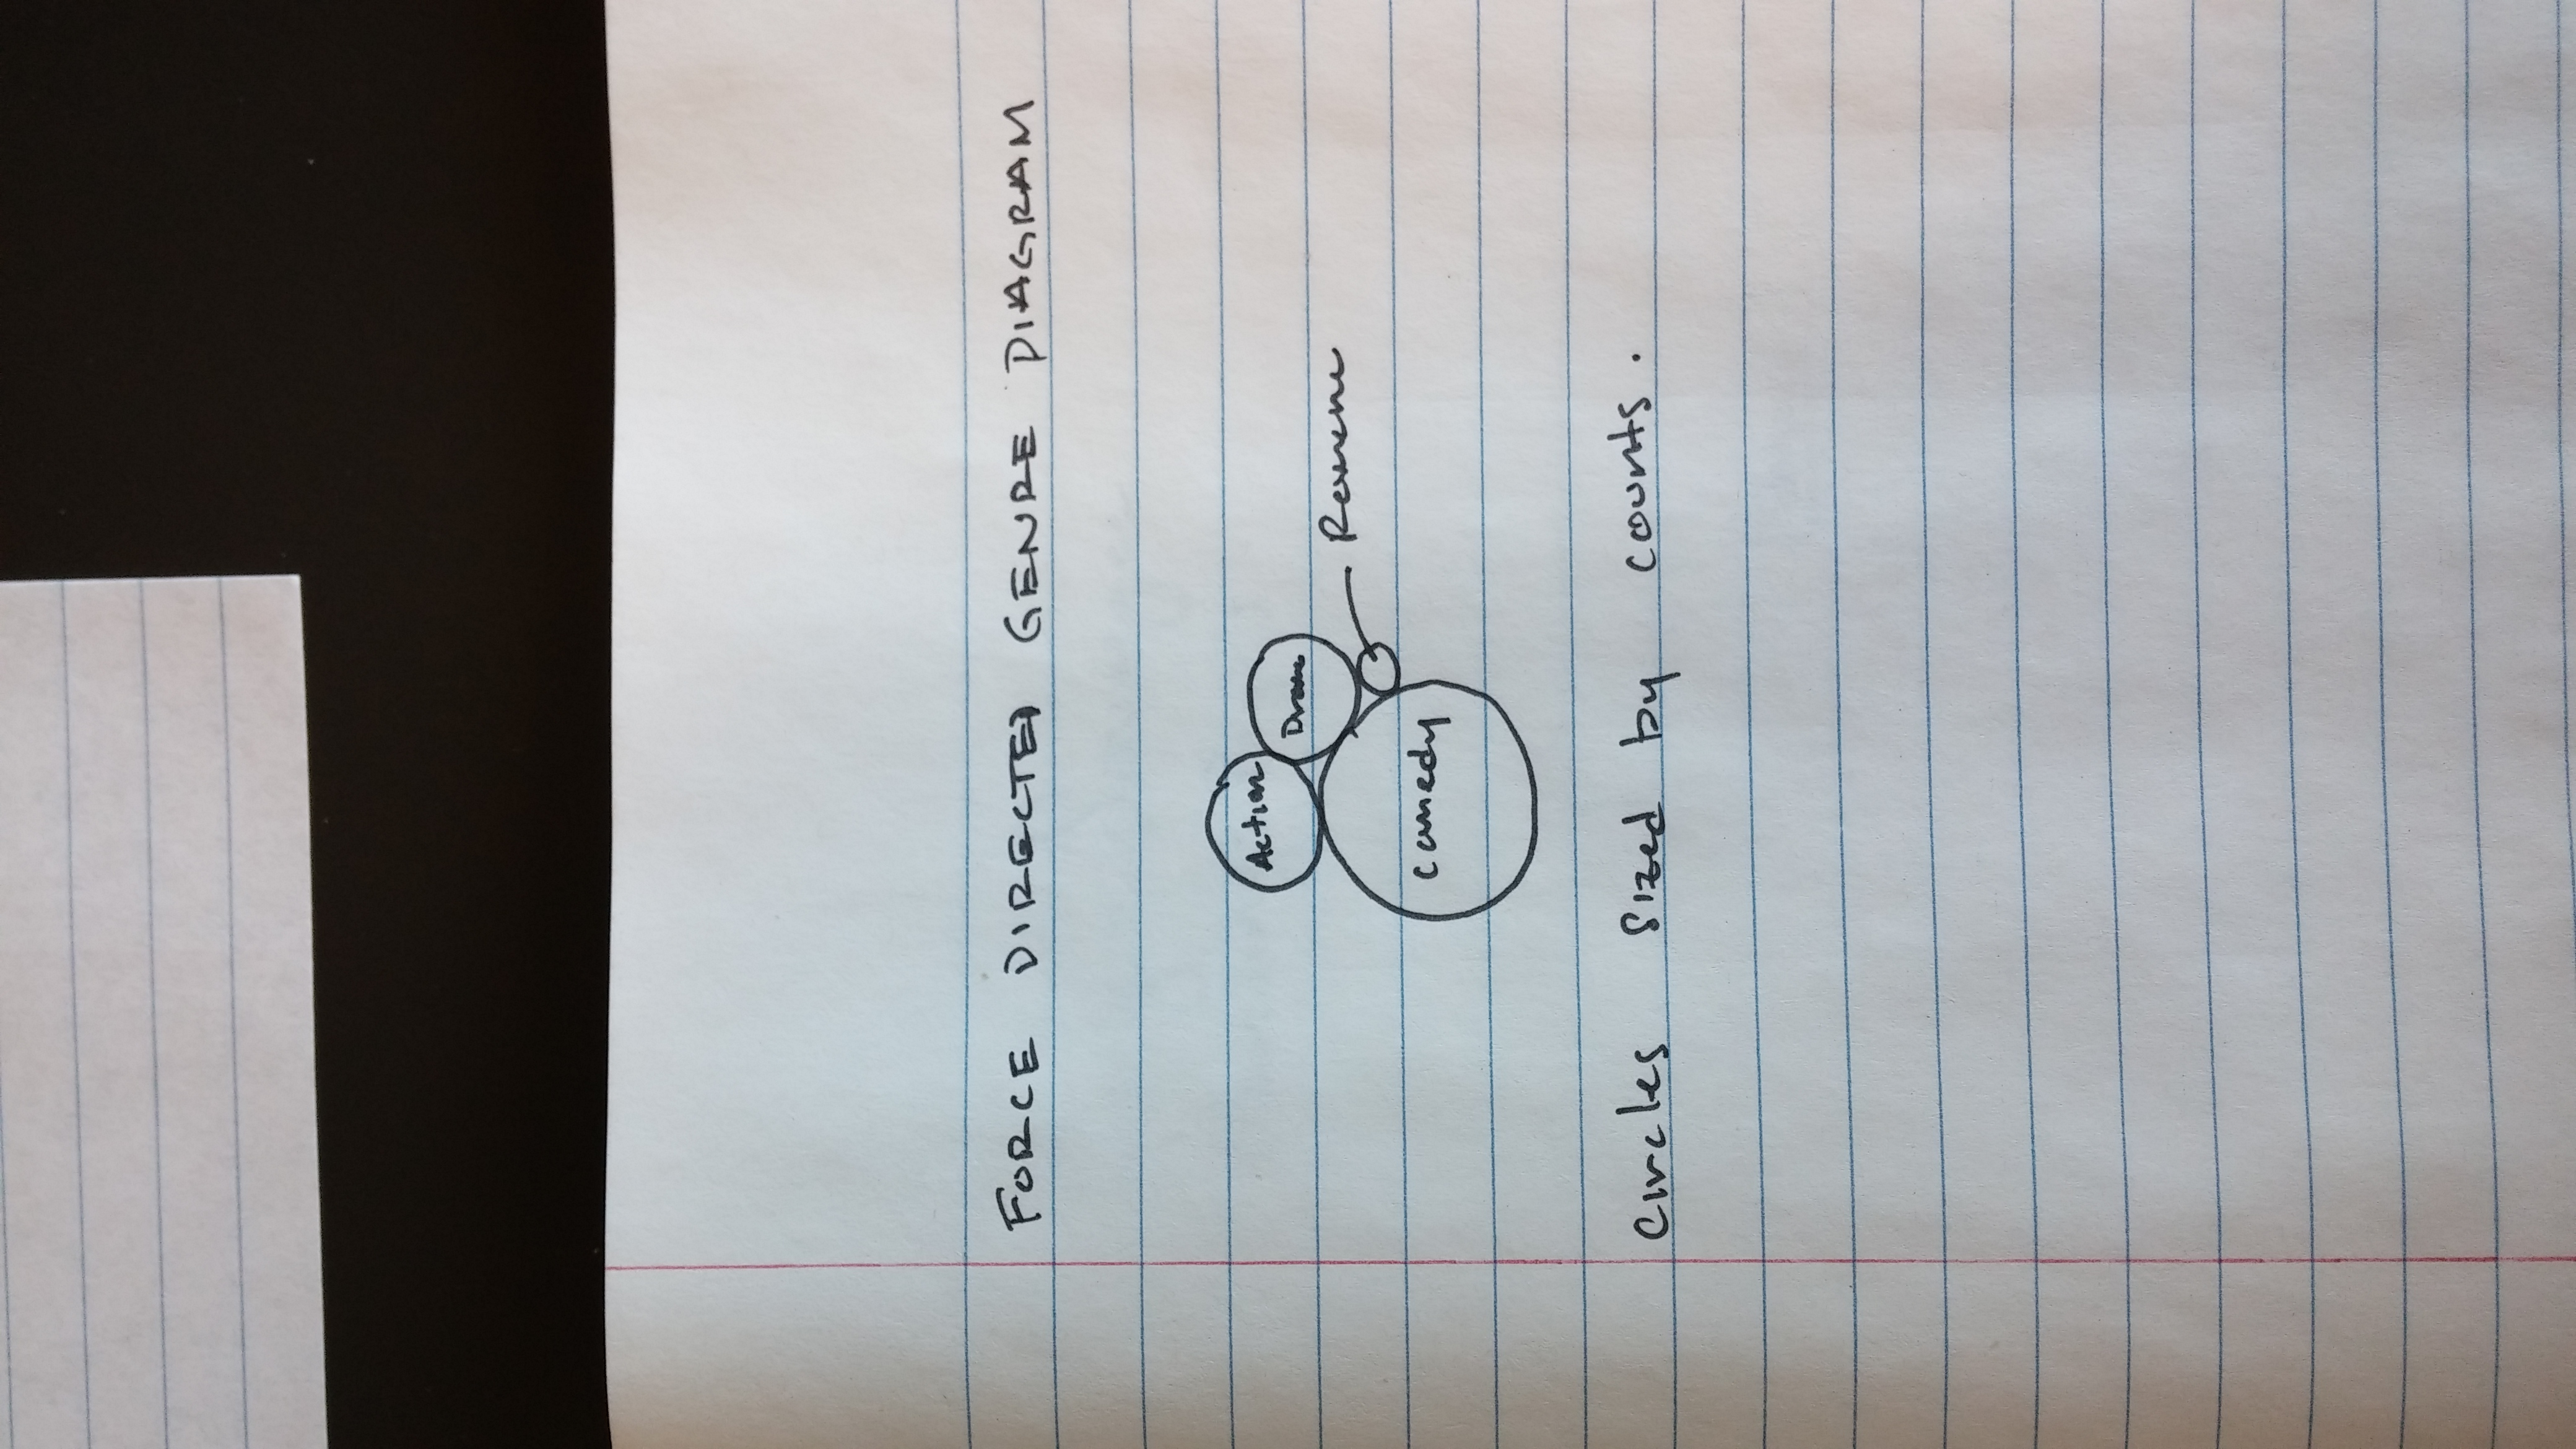
\includegraphics[angle=-90, scale=0.05]{force.jpg}
\end{center}
 This view shows an aggregate of all genres the selected actor has acted in over their career.  This view can quickly illustrate the actor's breadth of work in different areas.  Each circle corresponds to a single genre classification ('comedy', 'action', etc), and each genre receives a count for the number of films which use that as a descriptor. 
 
 

 
 \vspace{2em}
 
 \textbf{Mandatory Features}
 \begin{itemize}
  	\item Various genre classifications
  	\item highlight movies in Actor filmography timeline by selected/hovered genre.	
 \end{itemize}

\vspace{2em}
 
 \textbf{Optional Features}
\begin{itemize}
	\item N/A
\end{itemize}

\newpage 
\subsection{Extras}
\subsubsection{Income}
%\begin{center}
%\includegraphics[scale=•]{money.jpg}
%\end{center}

Create a scatter plot of the actors active years and plot annual income as reported through our data sources.

\subsubsection{Awards and Nominations}

Generate a barchart view (Stacked, based on nominations and awards).

\subsubsection{Co-actors}

Maintain an aggregated count of common actors which appear on screen with the selected actor.  This can be displayed as a Force diagram with each Node sized based on the number of times they appear with the selected actor.

\subsubsection{Actor as Other}

Change plots to show the Actor filmography in cases other than acting (ex. director, producer).

\newpage

\section{Project Schedule}
Plan your work so that you can avoid a big rush right before the final project deadline, and delegate different modules and responsibilities among your team members. Write this in terms of weekly deadlines.
\begin{center}
    \begin{tabular}{l l}
        \hline
        \textbf{Week} & \textbf{Goals and Milestones}\\
        \hline
        October 11 - 17				& Brain storm page layout data views \\
        October 18 - 24				& Set up web framework \\
        October 25 - 31				& Set up API calls/ error catching/ loading screens/ user experience \\
        November 1 - 7				& Wrangle data into workable model (start MVC) \\
        November 8 - 14 			& Begin views \\
        November 15 - 21			& Time-line view / testing \\
        November 22 - 28			& Graph view / testing	\\
        November 29 - December 4	& finalize views / testing \\
    \end{tabular}
\end{center}
\end{document}